\lecture{Controllo del Moto e Pianificazione delle Traiettorie nella Robotica Industriale}{14~-~06~-~2026}
%
%
\section{Il Controller come Traduttore Meccanico}
Questa sezione introduce il ruolo dell'unità di controllo e il concetto di traiettoria inteso come bilanciamento tra requisiti operativi opposti.
\begin{description}
    \item [Il Processo di Traduzione] Il controllore del robot agisce come un vero e proprio ``cervello'', con il compito di orchestrare un sistema cinematico complesso. Traduce i comandi ad alto livello impartiti dall'utente nella realtà fisica delle rotazioni dei singoli motori, calcolando tramite formule matematiche complesse i valori esatti di tensione e coppia necessari per ciascun attuatore.
    \item [Scelta della Traiettoria come Gestione del Rischio] La selezione del tipo di movimento non è puramente formale, ma rappresenta un calcolato compromesso (trade-off) tra velocità di esecuzione, precisione spaziale e sicurezza operativa. Una pianificazione errata o superficiale delle traiettorie costituisce la causa primaria delle cosiddette "collisioni fantasma" (urti imprevisti dovuti a percorsi non lineari) e dell'accelerata usura meccanica dei componenti.
\end{description}

%
\section{Dicotomia Fondamentale: Joint vs Cartesian}
\begin{itemize}
    \item \textbf{Spazio dei Giunti (Joint Space - Logica del Robot)}: In questa configurazione, lo stato e la posizione del robot sono definiti unicamente ed esclusivamente attraverso i singoli angoli o estensioni dei suoi giunti (es. Spalla: $45^\circ$, Gomito: $90^\circ$). Muoversi in questo spazio consente di massimizzare l'efficienza meccanica del manipolatore.
    \item \textbf{Spazio Cartesiano (Cartesian/Task Space - Logica Umana)}: La posizione e l'orientamento dello strumento sono descritti utilizzando i tradizionali assi tridimensionali ortogonali ($X, Y, Z$) espressi in millimetri. Questa modalità forza il robot a seguire specifici percorsi geometrici nello spazio, ignorando la naturale configurazione dei suoi motori.
\end{itemize}
Vedi figura \ref{fig:jvcs}.

\begin{figure}
    \centering
    \begin{subfigure}{0.45\linewidth}
        \centering
        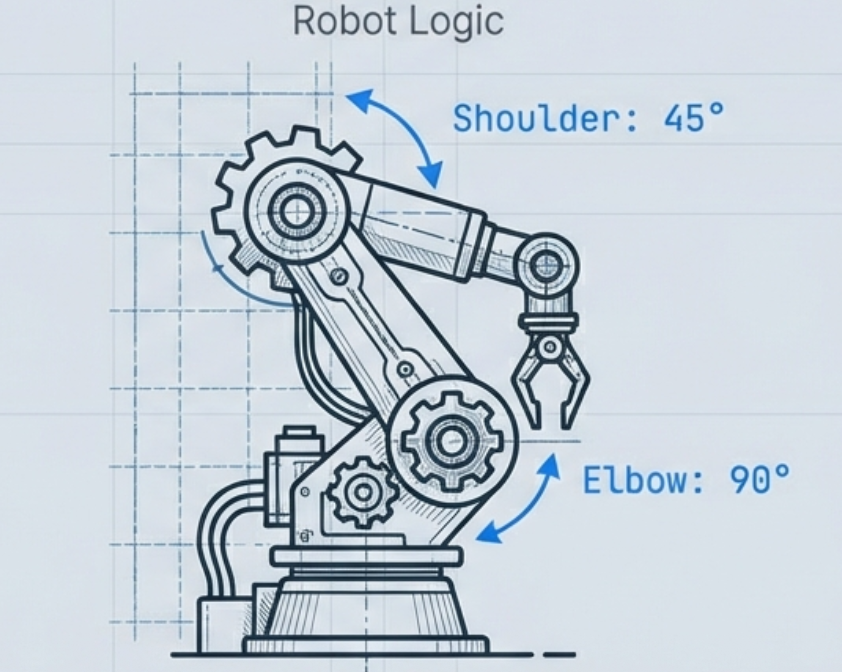
\includegraphics[width=\linewidth]{assets/jvc1.png}
        \caption{Joint Space}\label{fig:js}
    \end{subfigure}
    \begin{subfigure}{0.45\linewidth}
        \centering
        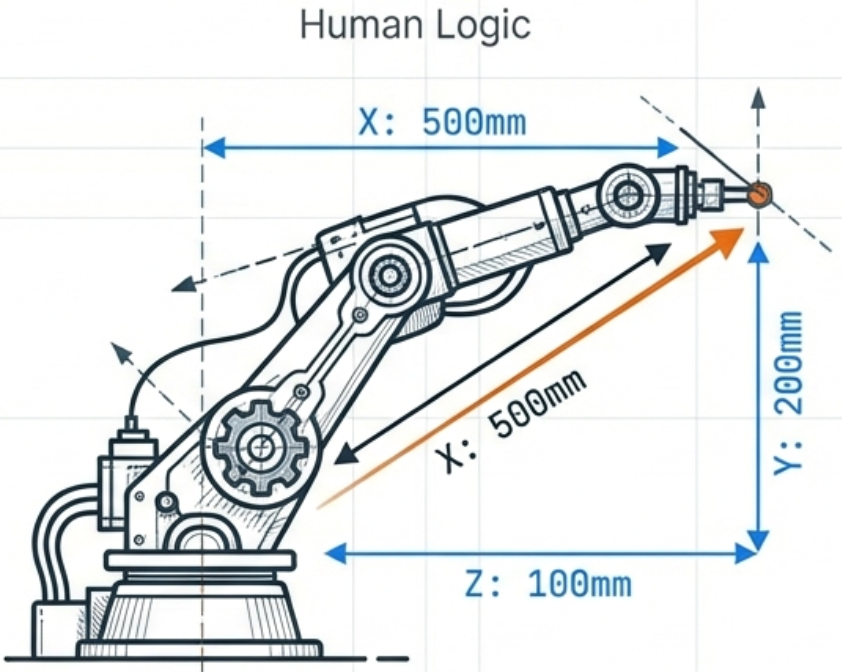
\includegraphics[width=\linewidth]{assets/jvc2.png}
        \caption{Cartesian Space}\label{fig:cs}
    \end{subfigure}
    \caption{Joint vs Cartesian Space}\label{fig:jvcs}
\end{figure}

%
\section{Analisi Comparativa dei Comandi di Movimento}
Questa sezione rappresenta il nucleo principale dell'analisi e descrive i quattro comandi standard di movimentazione industriale.
%
\subsection{MoveJ (Joint Motion)}
\begin{description}
    \item [Meccanica del Moto] Definito lo ``Sprinter'' dei movimenti, il controllore esegue un'interpolazione lineare direttamente sugli angoli dei giunti. Calcola un percorso ottimizzato in cui tutti i motori iniziano e terminano le proprie rotazioni nello stesso identico istante.
    \item [Vantaggi Tecnici] È il movimento cinematicamente più naturale ed efficiente dal punto di vista energetico, poiché consente di sfruttare le massime velocità operative permesse dai motori.
    \item [Applicazione Ideale] Spostamenti in aria (Air-moves), ovvero i trasferimenti rapidi attraverso spazi vuoti in cui non vi è alcuna interazione o contatto con l'ambiente o con i pezzi in lavorazione.
    \item [Il Pericolo Nascosto (Path Unpredictability)] Poiché \emph{MoveJ} ottimizza l'efficienza dei giunti e non il percorso nello spazio, la traiettoria finale del punto di riferimento dell'utensile (TCP) è un semplice ``sottoprodotto''. Il TCP descrive una curva complessa e non lineare, visivamente molto difficile da prevedere per un operatore umano, innalzando drasticamente il rischio di collisioni con ostacoli non mappati.
\end{description}
Vedi figura \ref{fig:movej}.
\begin{figure}
    \centering
    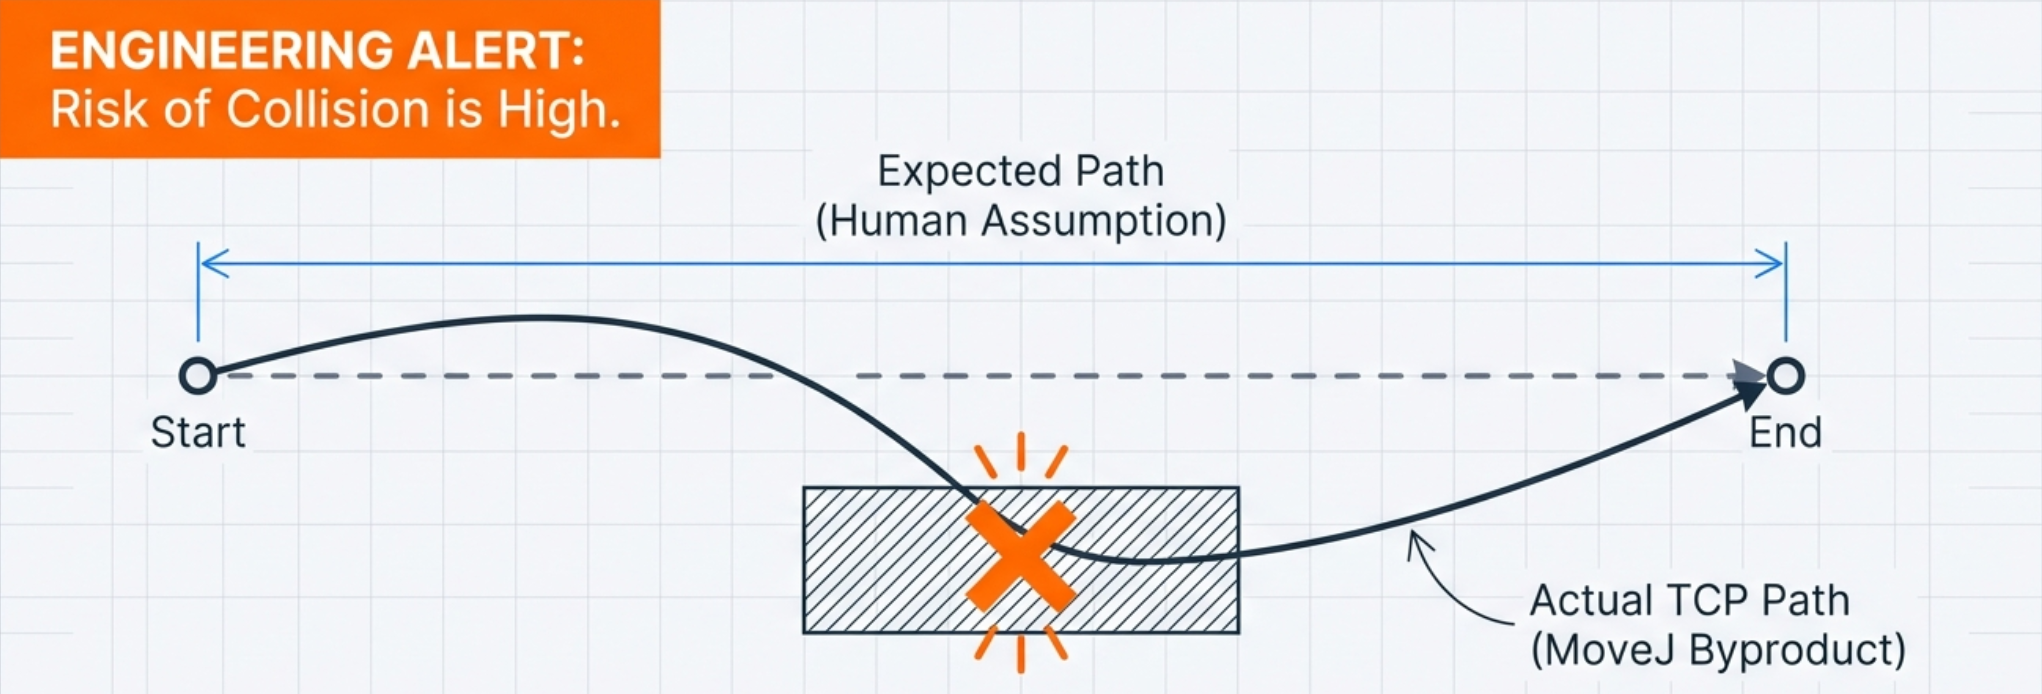
\includegraphics[width=\linewidth]{assets/movej.png}
    \caption{Path Unpredictability}\label{fig:movej}
\end{figure}
%
\subsection{MoveL (Linear Motion)}
\begin{description}
    \item [Meccanica del Moto] Conosciuto come il ``Chirurgo'', questo comando impone al TCP di seguire una linea retta perfetta e geometricamente definita tra il punto di partenza e l'arrivo.
    \item [Elevatissimo Carico Computazionale] Per contrastare le naturali curve della struttura e mantenere la linearità perfetta nello spazio cartesiano, il controllore deve risolvere in tempo reale i sistemi di equazioni della Cinematica Inversa (IK) a frequenze elevatissime, tipicamente comprese tra $125\si{Hz}$ e $500 \si{Hz}$. Il sistema esegue continuamente cicli di controllo per verificare e correggere gli angoli dei giunti centinaia di volte al secondo.
    \item [Applicazioni Ideali] Operazioni tecnologiche di processo in cui la traiettoria rettilinea è un vincolo non negoziabile, come saldatura, erogazione di colla, o assemblaggi meccanici di precisione.
    \item [Il Tallone d'Achille (Le Singolarità)] Il rischio principale di MoveL risiede nelle Singolarità Cinematiche, ovvero ``zone morte'' matematiche in cui gli assi si allineano o i giunti raggiungono i propri limiti fisici. In queste condizioni il software fallisce nel calcolo della cinematica inversa, provocando l'arresto immediato e abrupto del robot.
\end{description}
%
\subsection{MoveC (Circular Motion)}
\begin{description}
    \item [Meccanica del Moto] Consente di descrivere traiettorie circolari o curvilinee esatte e richiede la definizione obbligatoria di tre punti distinti: la posizione corrente ($P_1$), un punto di passaggio intermedio (ViaPoint, $P_2$) che determina matematicamente il raggio dell'arco, e il punto finale ($P_3$).
    \item [Sfumatura dell'Orientamento] Durante la traiettoria, il controllore sfuma l'orientamento angolare in modo continuo partendo dal punto iniziale direttamente verso l'EndPoint. Di conseguenza, non ci si deve aspettare che l'utensile rimanga perpendicolare alla superficie nel punto intermedio ($P_2$), a meno che questo non venga esplicitamente imposto e calcolato nei vettori di posa.
\end{description}
%
\subsection{MoveP (Process Motion)}
\begin{description}
    \item [La Caratteristica Distintiva] A differenza di MoveL o MoveJ (dove la velocità subisce fluttuazioni dovute alle rampe di accelerazione e decelerazione in prossimità dei punti di svolta), MoveP è progettato per mantenere una velocità cartesiana costante dell'utensile lungo tutto il percorso.
    \item [Applicazione] Risulta fondamentale per applicazioni industriali di finitura superficiale o deposizione uniforme di materiali (es. verniciatura a spruzzo o incollaggio continuo). Spesso integra al suo interno comandi MoveC per gestire in modo fluido e a velocità costante gli angoli curvi.
\end{description}
\begin{figure}
    \centering
    \begin{subfigure}{.9\linewidth}
        \centering
        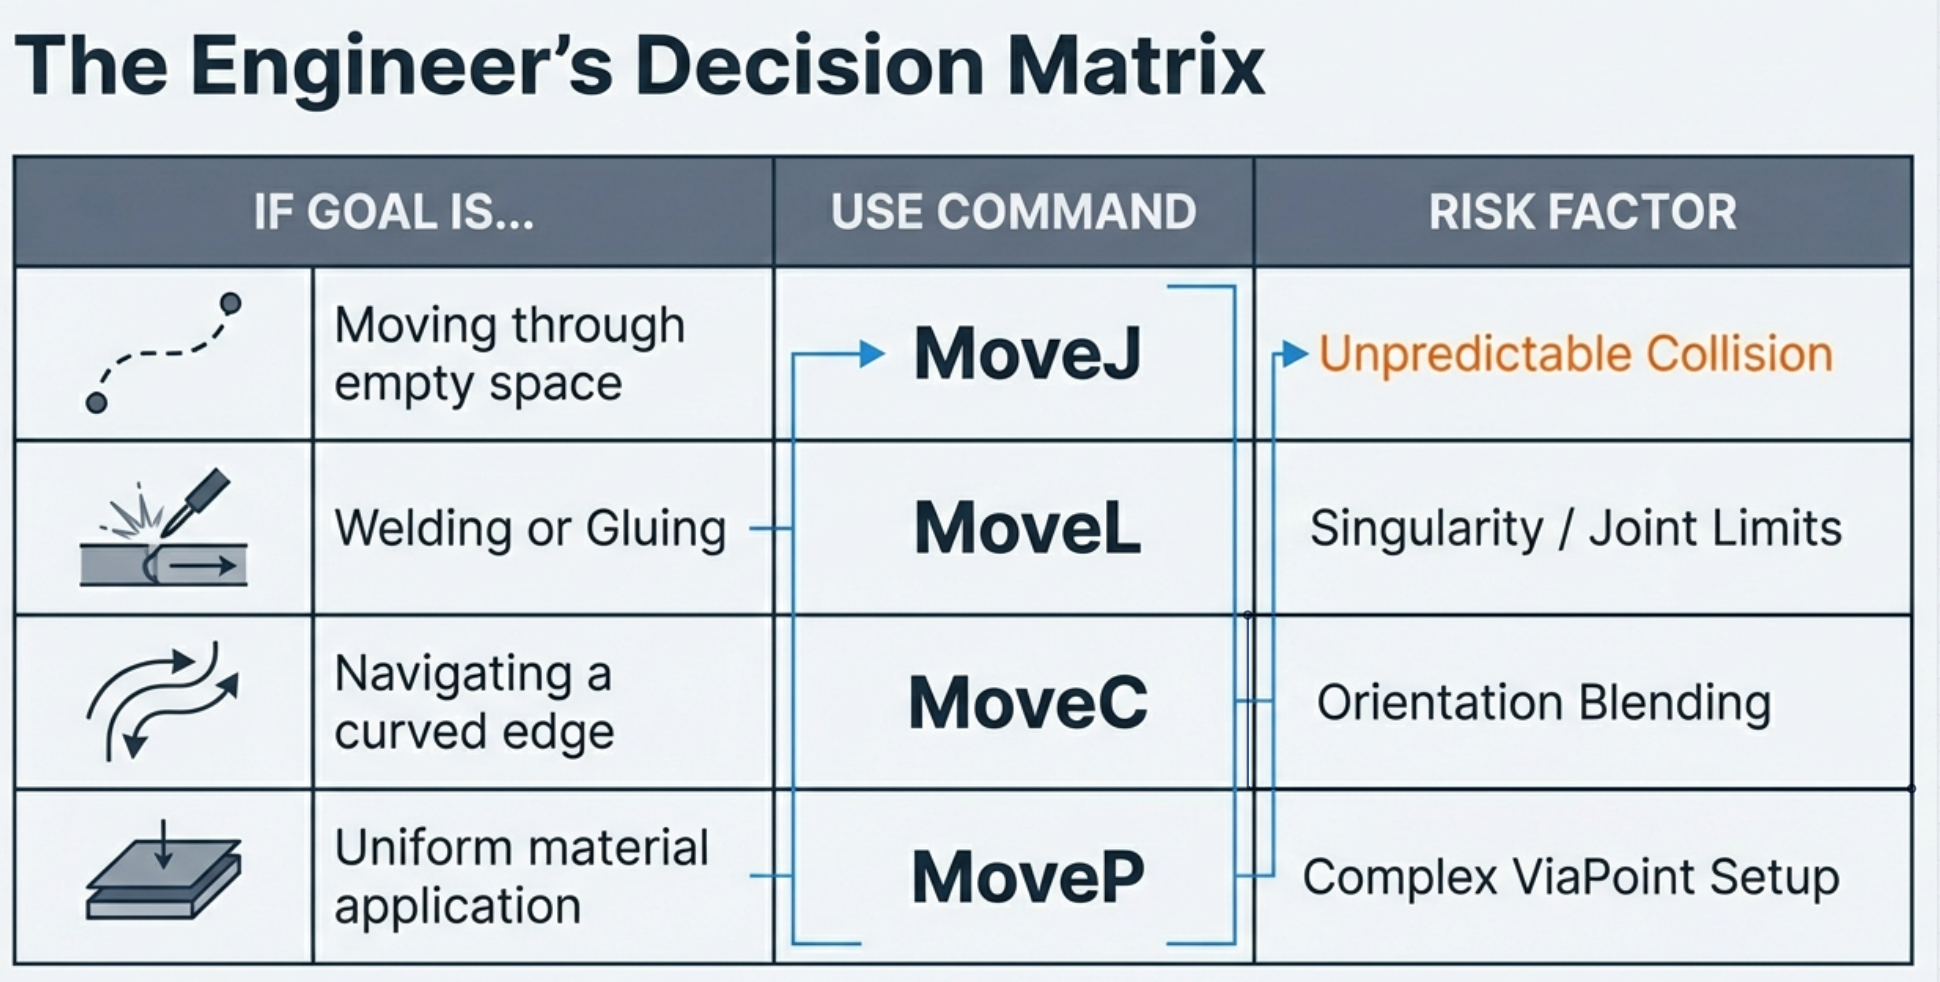
\includegraphics[width=\linewidth]{assets/movedec.png}
        \caption{Engineer's Decision Matrix}\label{fig:}
    \end{subfigure}
    \begin{subfigure}{0.9\linewidth}
        \centering
        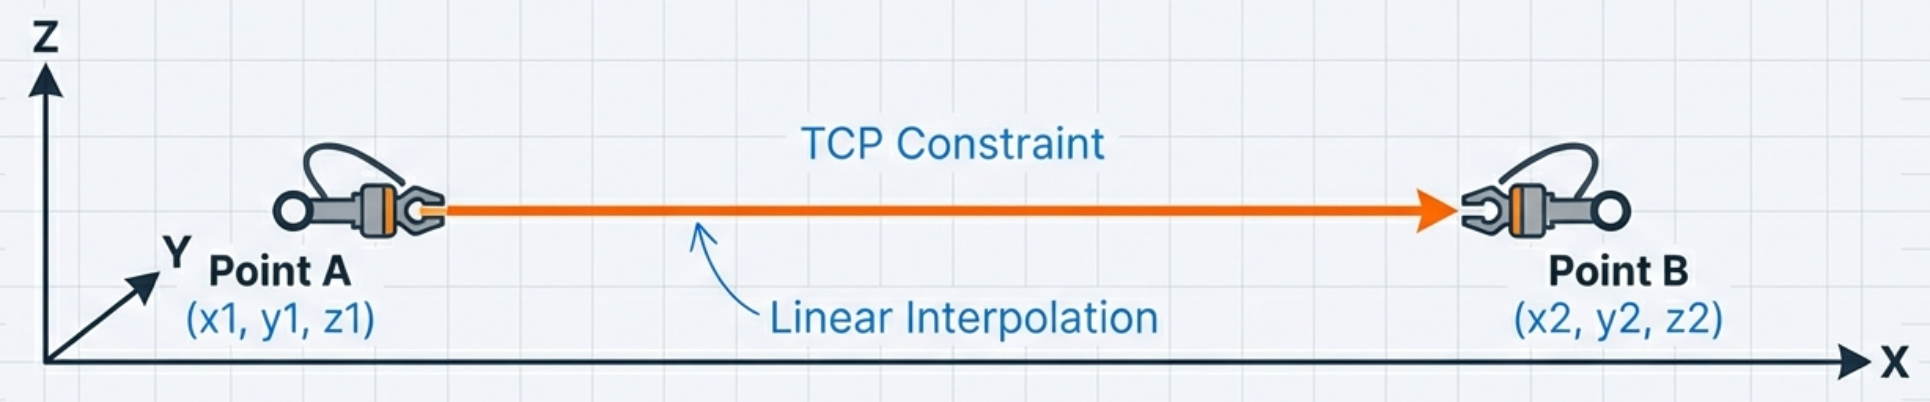
\includegraphics[width=\linewidth]{assets/movel.png}
        \caption{MoveL}\label{fig:}
    \end{subfigure}
    \begin{subfigure}{0.4\linewidth}
        \centering
        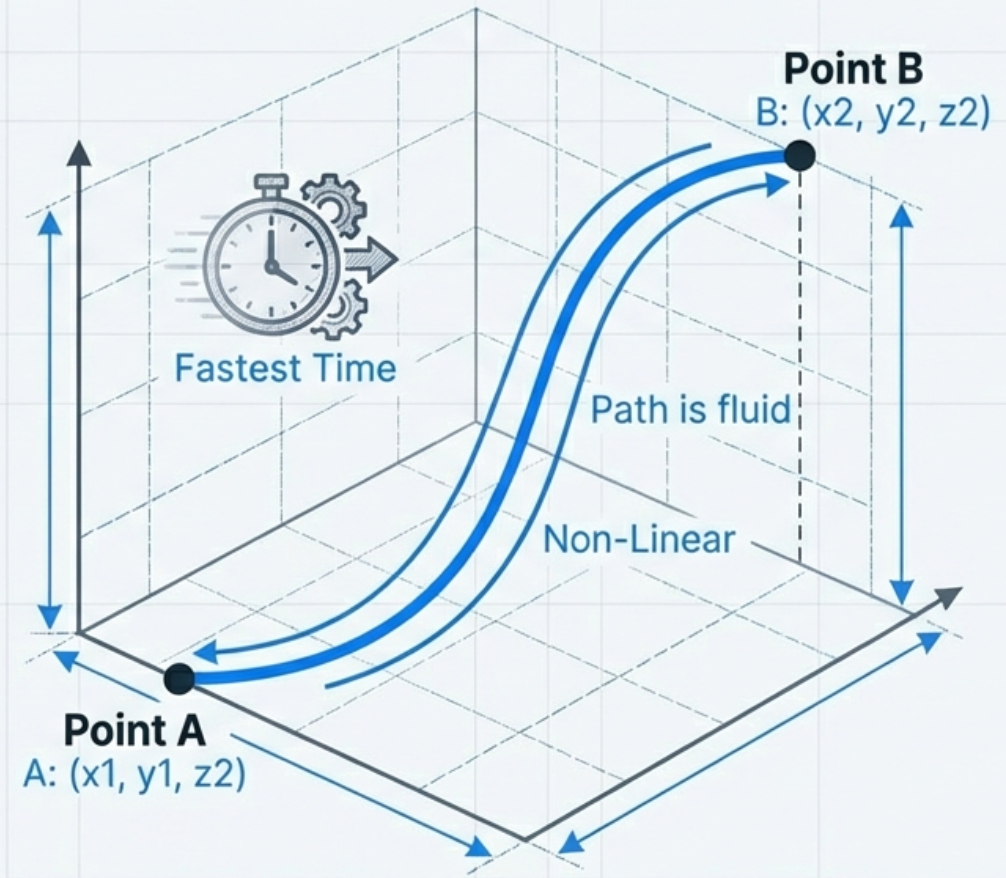
\includegraphics[width=\linewidth]{assets/movec1.png}
        \caption{MoveJ}\label{fig:}
    \end{subfigure}
    \begin{subfigure}{0.5\linewidth}
        \centering
        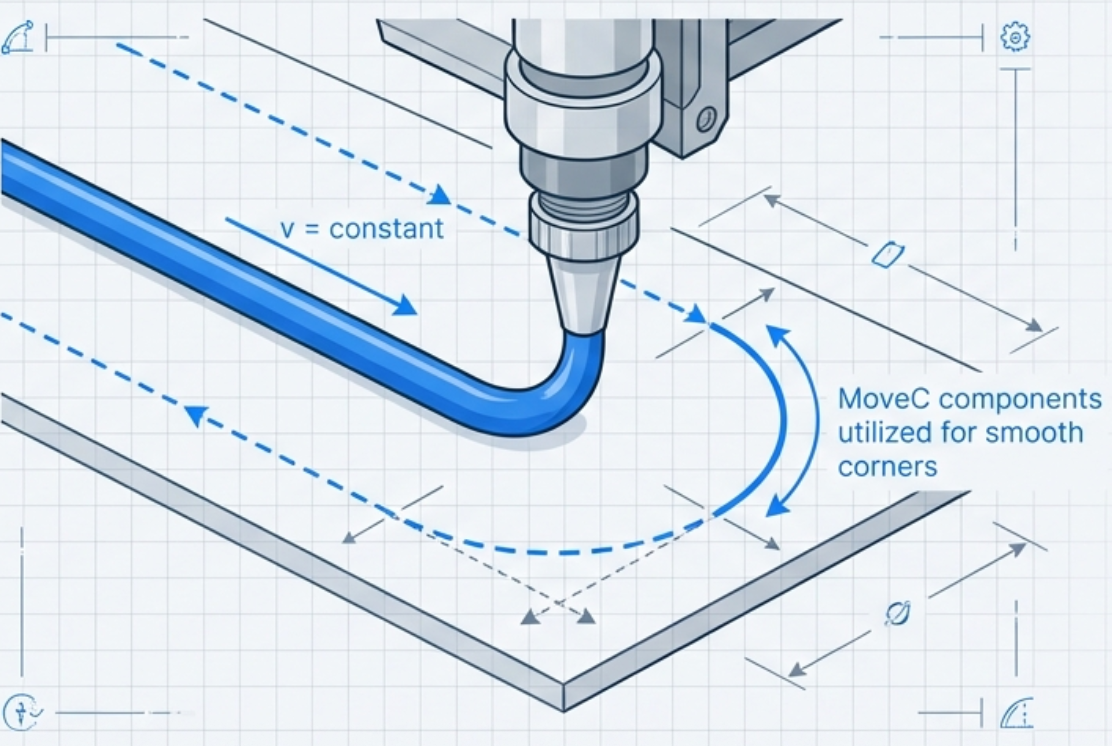
\includegraphics[width=\linewidth]{assets/movep.png}
        \caption{MoveP}\label{fig:}
    \end{subfigure}
    \begin{subfigure}{0.45\linewidth}
        \centering
        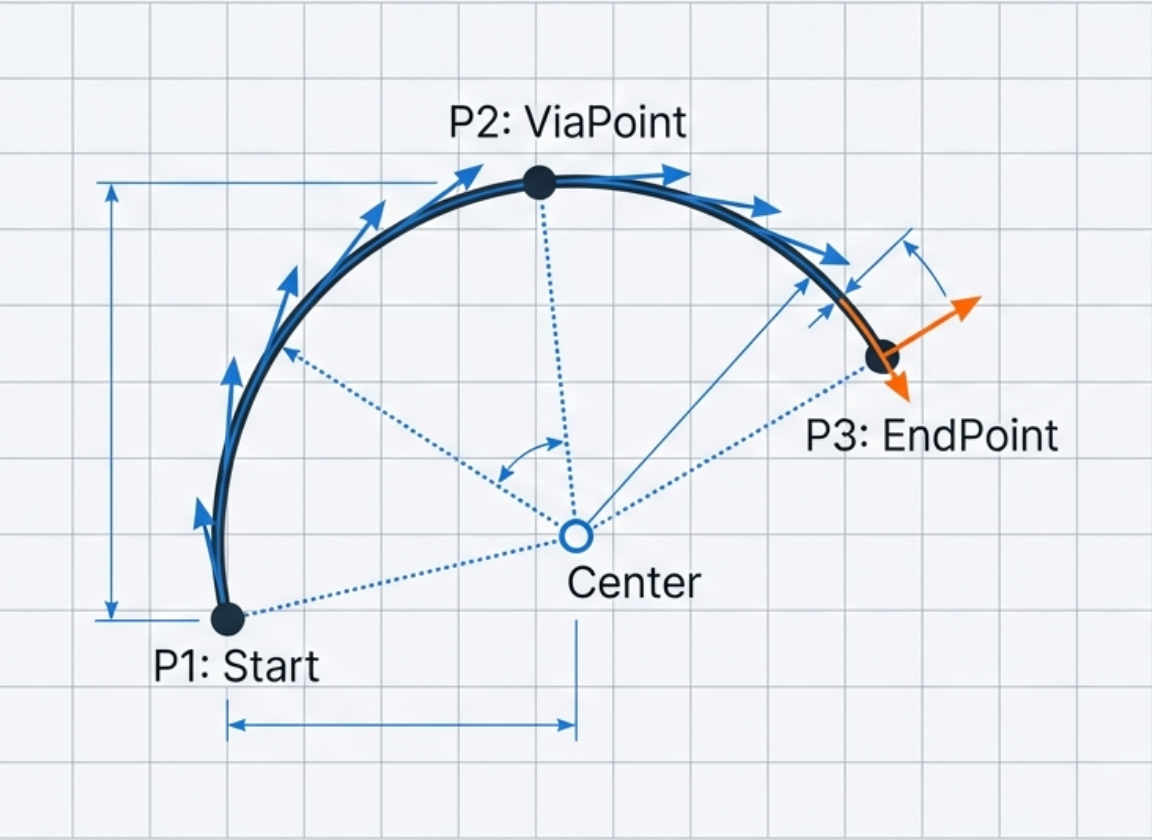
\includegraphics[width=\linewidth]{assets/movec.png}
        \caption{MoveC}\label{fig:}
    \end{subfigure}
    \caption{}\label{fig:}
\end{figure}
